\section{化合物半导体的能带结构}
\Romnum{3}--\Romnum{5}族化合物半导体与硅和锗具有同一类型的能带结构,这是因为\Romnum{3}--\Romnum{5}族化合物的闪锌矿结构和金刚石结构类似,因此简约布里渊区均为截角八面体,故价带和导带也是相似的
\begin{itemize}
    \item \Romnum{3}--\Romnum{5}族化合物的价带与硅和锗类似,价带在布里渊区域的中心简并,并同样具有一个重空穴和一个轻空穴,以及一个由自旋--轨道耦合而分裂出来的第三能带,但是,价带的极小值往往并不是恰好位于布里渊区的正中心,而是稍微有些偏离,但偏离的不多。
    \item \Romnum{3}--\Romnum{5}族化合物的导带比较多样,在$[100]$和$[111]$以及布里渊区中心均有极小值,但是取决于化合物的具体类型,其中最小的极小值的出现位置可能不同,具体而言
    \begin{itemize}
        \item 若平均原子序数较小,则导带最小值出现在布里渊区的中心。
        \item 若平均原子序数较大,则导带最小值出现在$[100]$和$[111]$方向。
    \end{itemize}
    \item 各化合物中,价带的重空穴有效质量差异不大,而平均原子序数越高,导带电子的有效质量越小,同时,禁带宽度也越窄,事实上,禁带宽度最短的\Romnum{3}--\Romnum{5}族化合物中,由于价带和导带距离太近,两者间甚至会发生相互作用,使得极值处不再呈现抛物线形状。
\end{itemize}

这里我们重点介绍两种\Romnum{3}--\Romnum{5}族化合物:砷化镓(\ce{GeAs})、锑化铟(\ce{InSb})。

砷化镓的导带极小值位于布里渊区中心$\vb*{k}=\vb*{0}$,这与价带极大值在$\vb*{k}$上是相重合的,所以我们说,\empx{砷化镓是一种直接带隙半导体},区别于\xref{sec:硅和锗的能带结构}中,\empx{硅和锗是间接带隙半导体},砷化镓的能带结构如\xref{fig:砷化镓的能带结构}所示,从图中我们能形象的看出,砷化镓的导带其实在$\<100>$和$\<111>$以及布里渊区中心均有极小值,只不过布里渊区中心处为最小值,在$\<111>$方向(点$L$)的较高能谷比在布里渊区中心(点$\Gamma$)的较低能谷的高了约$0.29\si{eV}$,并且我们可以注意到,砷化镓的价带中重空穴对应的曲线的极大值确实如前面提到的那样,略微了偏离了布里渊区的中心。

\begin{Figure}[砷化镓的能带结构]
    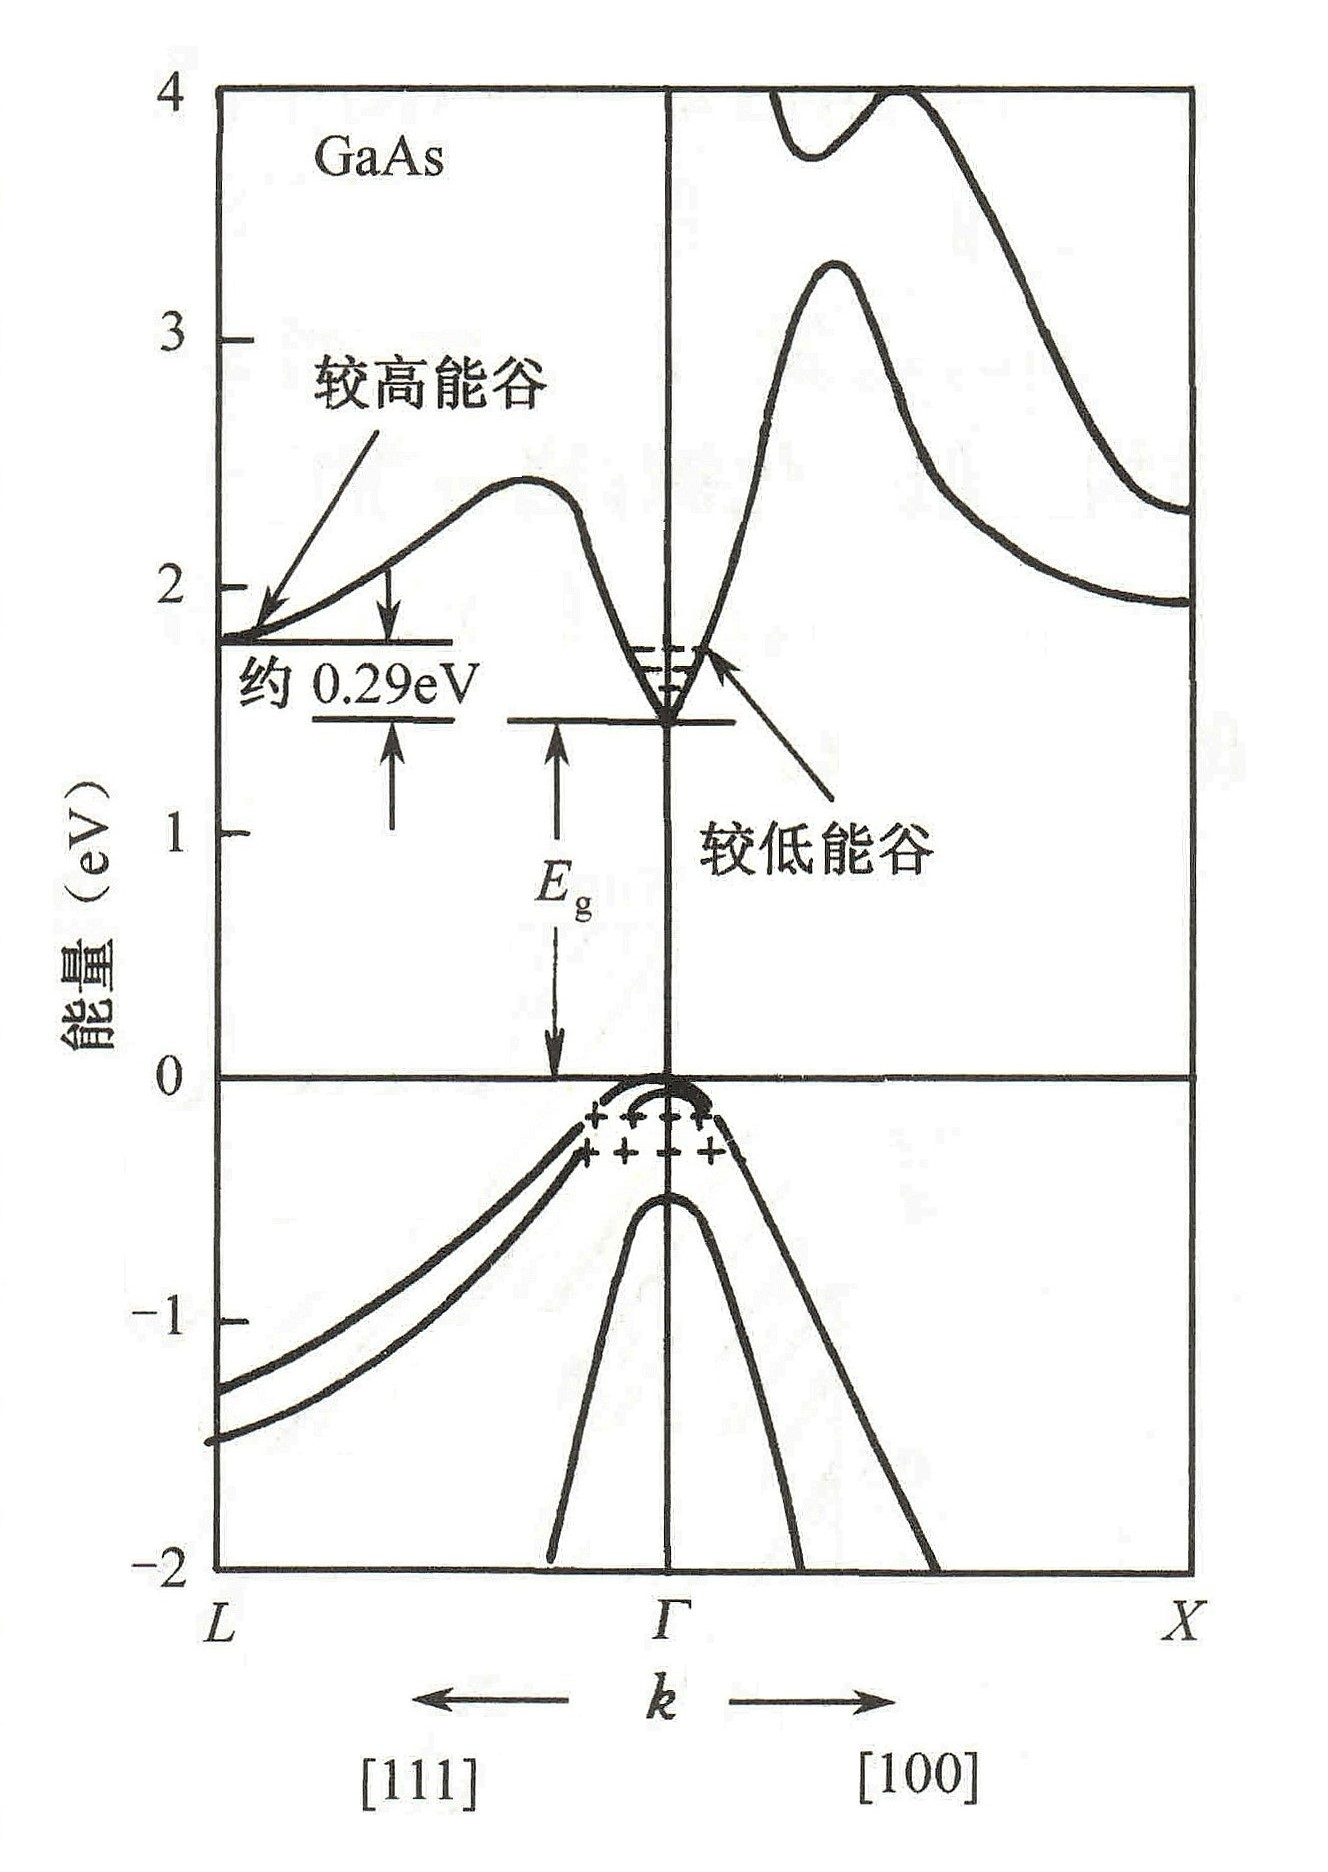
\includegraphics[width=6cm]{image/GaAs_Band.jpg}
\end{Figure}

锑化铟也是直接带隙半导体,但需要特别说明的是,锑化铟的禁带宽度很窄,故能带是非抛物线形的,并且,锑化铟的重空穴的极大值偏离布里渊区中心相对较大(只是相对其他化合物而言,仍然很小),极大值在$\vb*{k}$方向上位于布里渊区中心和布里渊区边界间$0.3\%$的位置,极大值的能值高出了$10^{-4}\si{eV}$,因此,锑化铟的重空穴在不同方向的有效质量$(m_\text{p})_\text{h}$是不同的。

\begin{Table}[部分半导体材料的参数]{ccccccccc}
    <
    \mrx<c>{3}{材料}&
    \mc{2}(c){电子有效质量$\mne$}&
    \mc{3}(c){空穴有效质量$\mpe$}&
    \mrx<c>{2}{裂距}&
    \mrx<c>{2}{禁带宽度\footnotemark}&
    \mrx<c>{2}{导带极小值}\\
    &纵向&横向&重&轻&第三\\
    &$m_l$&$m_t$&$(m_\text{p})_\text{h}$&$(m_\text{p})_\text{l}$&$(m_\text{p})_3$&$\Delta$&$E_\text{g}$&--\\
    >
    硅&$0.98m_0$&$0.19m_0$&$0.53m_0$&$0.16m_0$&$0.245m_0$&$0.04\si{eV}$&$1.14\si{eV}$&$X$\quad $\<100>$方向\\
    锗&$1.64m_0$&$0.08m_0$&$0.28m_0$&$0.044m_0$&$0.077m_0$&$0.29\si{eV}$&$0.67\si{eV}$&$L$\hspace{0.25em}\quad $\<111>$方向\\
    砷化镓&\mc{2}(c){0.063$m_0$}&$0.50m_0$&$0.076m_0$&--&$0.34\si{eV}$&$1.52\si{eV}$&$\Gamma$\quad$\vb*{k}=\vb*{0}$\\
    磷化镓&$0.91m_0$&$0.25m_0$&$0.67m_0$&$0.17m_0$&--&--&$2.27\si{eV}$&$X$\quad$\<100>$方向\\
    磷化铟&\mc{2}(c){$0.073m_0$}&$0.45m_0$&$0.12m_0$&--&--&$1.34\si{eV}$&$\Gamma$\quad$\vb*{k}=\vb*{0}$\\
    \hspace*{0.4em}锑化铟\footnotemark&\mc{2}(c){$0.012m_0$}&$0.44m_0$&$0.016m_0$&--&$0.9\si{eV}$&$0.18\si{eV}$&$\Gamma$\quad$\vb*{k}=\vb*{0}$\\
\end{Table}

\footnotetext[1]{这里的禁带宽度是室温禁带宽度,因此硅和锗的数据与\xref{tab:硅和锗的禁带性质}中给出的绝对零度时的禁带宽度不同。}
\footnotetext[2]{锑化铟重空穴的有效质量是各向异性的,$[111]$方向为$0.44m_0$,$[110]$方向为$0.42m_0$,$[100]$方向为$0.32m_0$,表中取最大值。}

在\xref{tab:部分半导体材料的参数}中,整理列出了一些半导体材料的主要参数。